

%\documentclass[conference]{IEEEtran}
%\IEEEoverridecommandlockouts
\documentclass{article}  
\twocolumn

\usepackage{graphicx}
\usepackage{algorithm}
\usepackage{algorithmic}
\usepackage{amsmath}
\usepackage{adjustbox}
\usepackage{authblk}
\usepackage{pbox}
\usepackage{float}
\usepackage[margin=1in]{geometry}
\author[1]{Dalia Ibrahim}
\author[2]{Carlos Dasaed Salcedo}


{
    \makeatletter
    \renewcommand\AB@affilsepx{: \protect\Affilfont}
    \makeatother
        
        

    \affil[ ]{Studnet ID}

    \makeatletter
    \renewcommand\AB@affilsepx{, \protect\Affilfont}
    \makeatother

    \affil[1]{201893217}
    \affil[2]{201892008}
    
        \makeatletter
\setlength{\floatsep}{5pt}
\setlength{\textfloatsep}{5pt}
    \makeatother
    
}

\begin{document}  

\title{ Assignment 3: Choosing the Best Model Between KNN, Random Forest, and Logistic Regression for a Sample Binary Classification Test File}


\maketitle
 \section{Introduction}
For this assignment, we have implemented an algorithm that selects the best model between KNN, Random Forest, and Logistic Regression. Since the decision boundary of the test data is unknown, the methods selected were intended to cover most of the possible hypothesis spaces. KNN was selected because it is a simple method capable of adapting to complicated decision boundaries.  Random Forest was an obvious choice, as it doesn't suffer from over fitting, and it provides the added bonus of being able to rank the importance of the features. Logistic regression was chosen with the intend of having a primarily linear classifier, as it will perform better in case the decision boundary of data turns out to be linear. To run the program, the following line must be executed from the command line in Linux: \\
\$python3 A3.py [TrainingFile.tsv] [TestingFile.tsv]

\section{Data Pre-processing}
Random forest have an inherent ability that allows them to rank features according to their importance. Therefore, an initial function called Feature Selection \_RandomForest() was programmed to generate a temporary random forest classifier fitted with the training data. This temporary classifier is then tuned with bootstrap and the gini index as the criteria for feature selection. A variable called "importances" is used to store the sorted ranking order of the features. Since the column order of the training data needs to match the column order of the testing data, all the columns in the testing and training file are sorted according to the rankings stored in "importances". In other words, the pre-processing stages of the algorithm consists in sorting the columns of the training and testing files according to the gini index generated by the random forest library of SciKit learn.

\section{Range of Parameters}
Even though the training data is the same for all the models, they each use different variables and formulas to generate their predictions. For this reason, a different range of parameters had to be tuned according to the model in question. In the case of random forest, these were the parameters tuned:
\begin{itemize}
	\item Number of trees: Ranging from 200 to 2000
	\item Number of features(m): ${\sqrt{p}}$ or ${log_2(p)}$, where p is the number of features in the training data
	\item Number of leaves: Manually tested using trial and error
	\item Bootstrap set to True
\end{itemize}

In the case of logistic regression, the basic SciKit learn function was using its default values. In the case of KNN, the parameters were:
\begin{itemize}
	\item Number of neighbors (k)
	\item Number of features(m), where p is the number of features in the training data
\end{itemize}

Finally, as mentioned in the Data Pre-processing section, each of the models were ran with the features sorted, and unsorted. 


\section{KNN}
KNN is simple algorithm which generates its results from a majority vote of the closest neighbors to determine if an instance belongs to a particular class. Unfortunately, its results vary greatly based on the number of neighbors and  features to consider for the training of the model. Therefore, cross-validation was used to determine the optimal number of K-nearest neighbors and the number of features to select. This cross-validation process was ran twice, once with the training data unsorted, and once with the sorted training data. 

\begin{center}
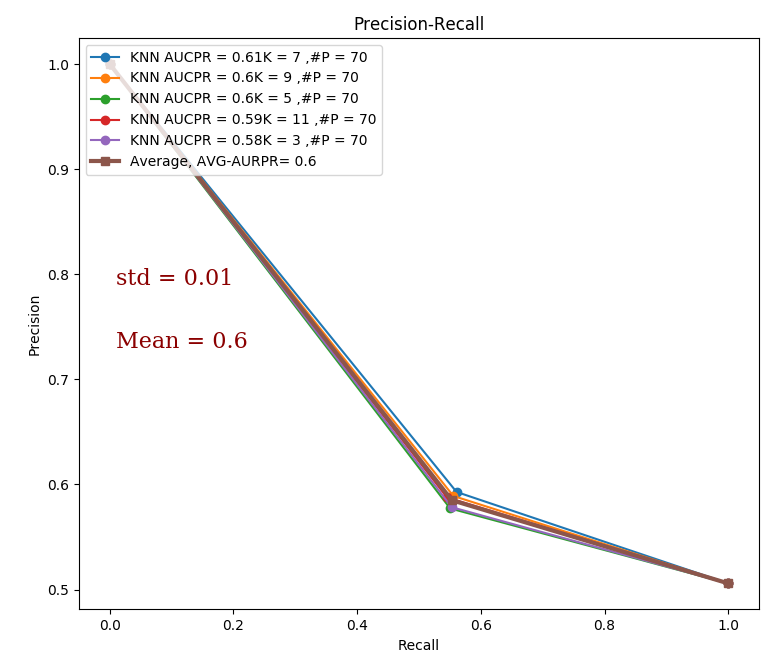
\includegraphics[scale=.25]{KNN_New.png} %{with .png} 
\end{center}
Fig. 1 KNN Precision-Recall Curve using sorted features\\

\begin{center}
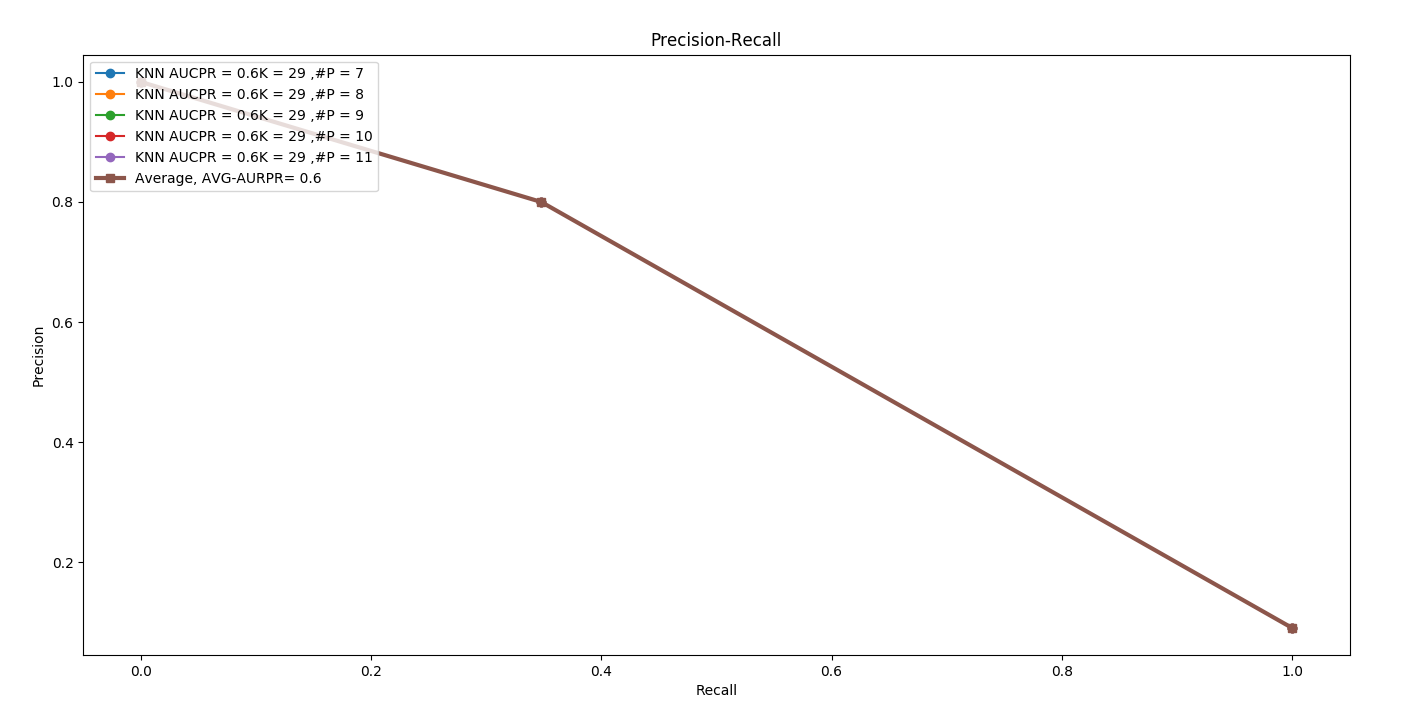
\includegraphics[scale=.17]{KNN_Withoutfeature.png} %{with .png} 
\end{center}
Fig. 2 KNN Precision-Recall Curve using unsorted features\\

As Figures 1 and 2 show, the order of the features did not have much of an impact on the performance of the algorithm, hence both graphs show similar results, and a mean AUCPR score of 61\%. However, the results of Figure 2 may be misleading, as the best results with the unsorted data suggest the use of 29 neighbors, implying that this KNN model might actually be suffering from over fitting. 

\section{Random Forest}
Random forest is a machine learning algorithm that generates multiple decision trees and then does majority vote among its multiple trees to decide on the best classification of an instance. However, cross validation still needs to be ran on the algorithm to determine an appropriate number of parameters to select. Figure 3 displays the best results obtained from the Random Forest models, while figure 4 displays the worst results obtained.

\begin{center}
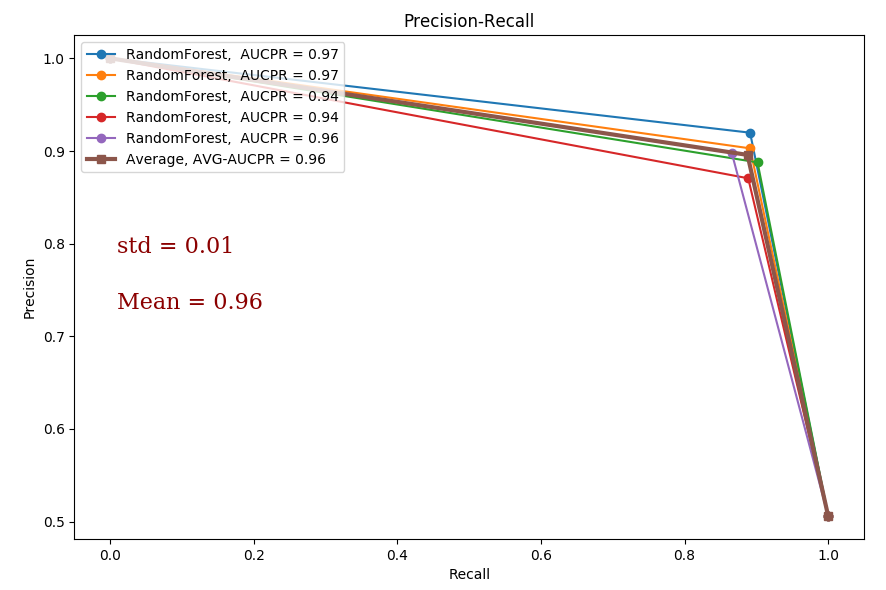
\includegraphics[scale=.25]{RandomForest_CV.png} %{with .png} 
\end{center}
Fig. 3 Random Forest best models and average AUCPR \\

\begin{center}
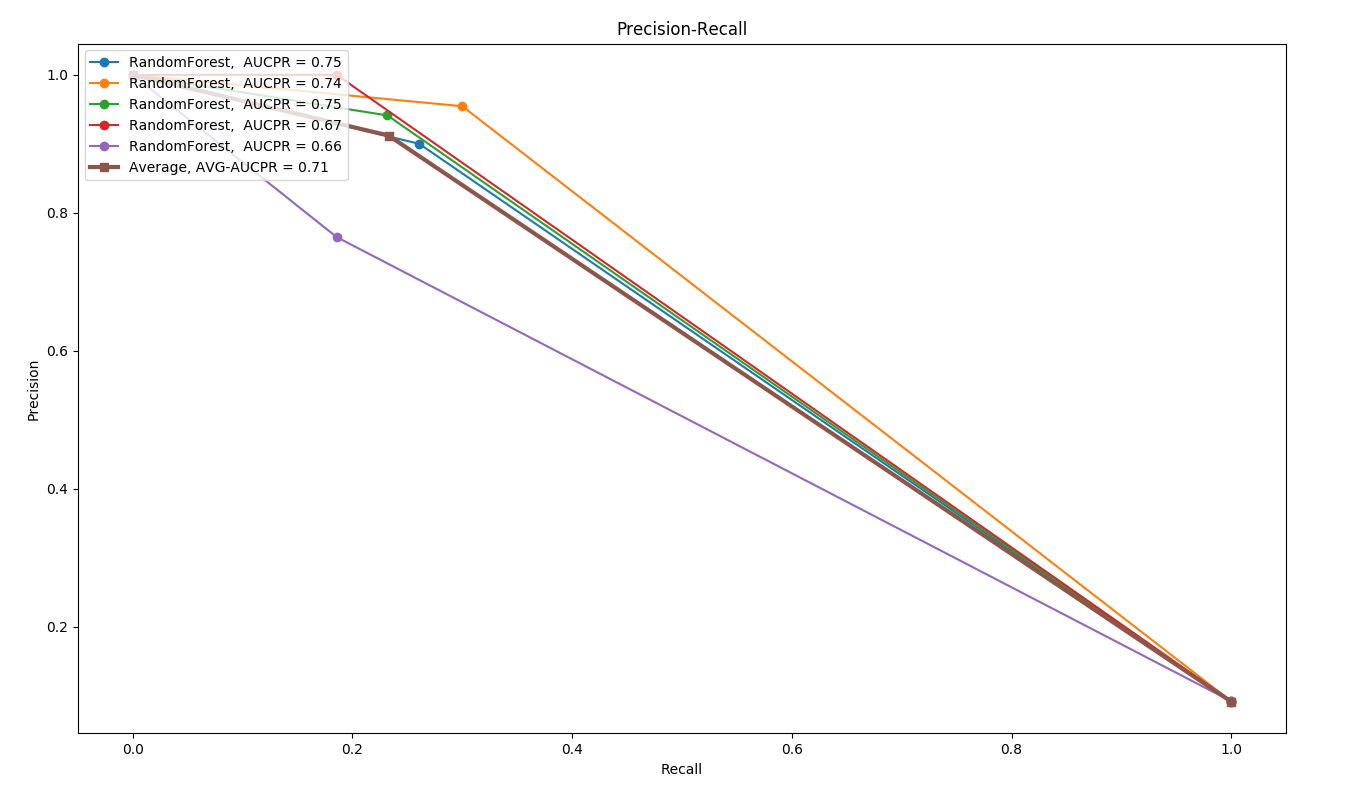
\includegraphics[scale=.17]{RF_WithoutOrdering.png} %{with .png} 
\end{center}
Fig. 4 Random Forest using unsorted features. \\

For random forest, the best model yielded a mean AUCPR score of 96\%, the highest out of all the models tested. 


\section{Logistic Regression}
As a linear model, logistic regression tends to be a popular method to use for binary classifiers. During the testing of the logistic regression models, incredibly poor results were obtained as seen in figure 5, to the point where even a program that randomly predicts the class of an instance would have performed better. However, applying the feature sorting mentioned in the data pre-processing section managed to help the model, and yield results with mean  AUCPR scores up to 88\%, as seen in figure 6. Even though the speed of the models to generate a result was not a criteria for the assignment, it is worth mentioning that logistic regression was the fastest in computing and outputting the results. 


\begin{center}
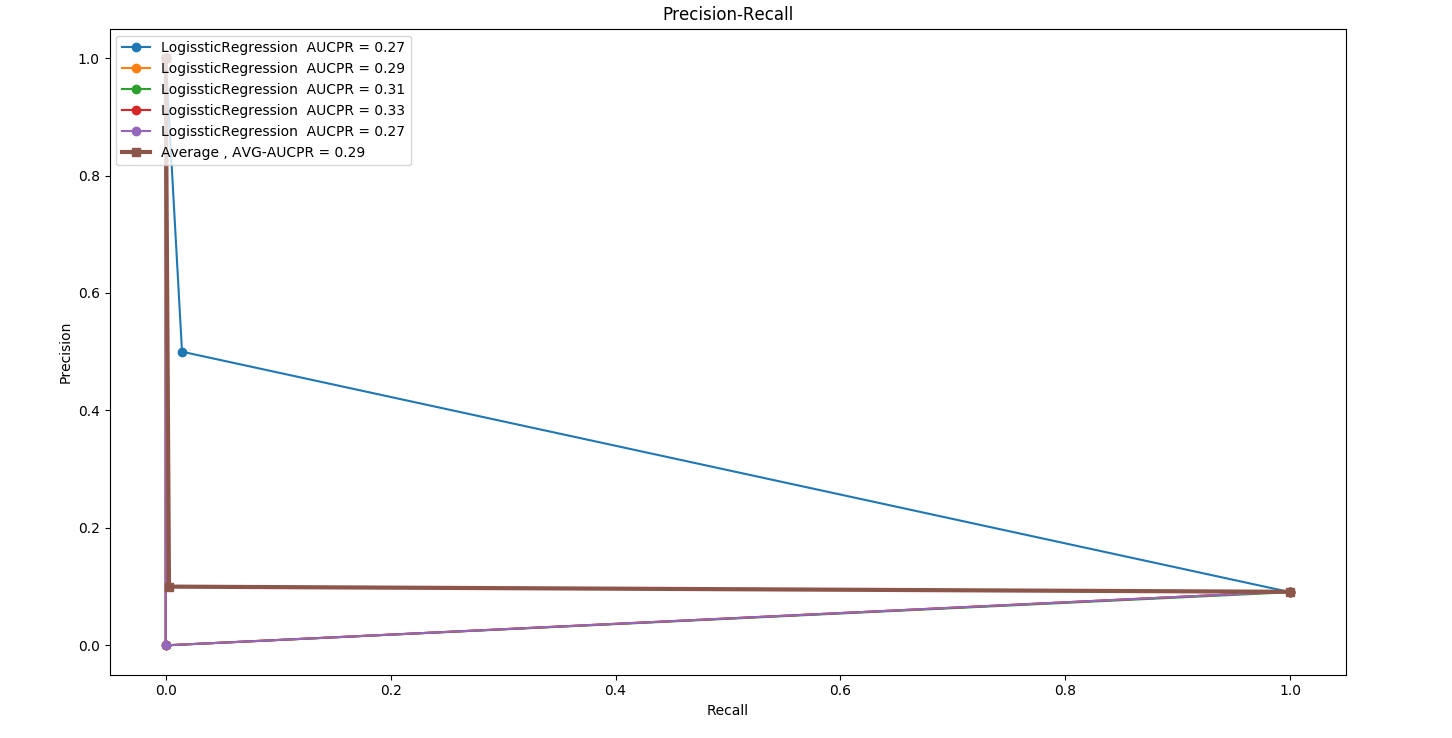
\includegraphics[scale=.17]{LOG_WithoutImp.png} %{with .png} 
\end{center}
Fig. 5 Logistic Regression without any data pre-processing steps \\

\begin{center}
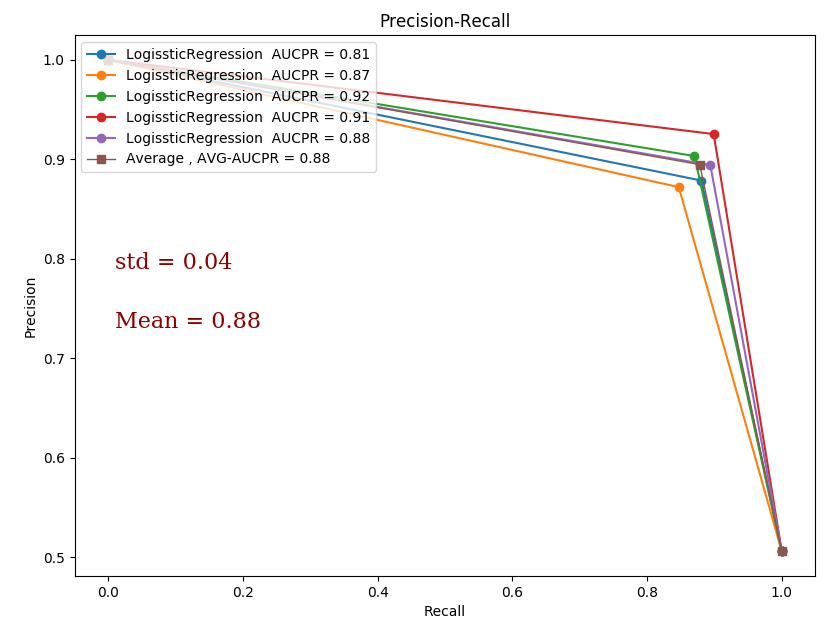
\includegraphics[scale=.25]{Logistic_CV.png} %{with .png} 
\end{center}
Fig. 6 Logistic Regression best models and average AUCPR \\

\section{Results}
Figure 7 provides a summary of the results obtained by the algorithm, as it shows the precision recall curves of the best model for each of the methods selected. The best KNN model was achieved with 7 neighbors and 70 ordered features. For random forest, the best model was achieved with the following parameters: bootstrap set to True, $log_2$ number of parameters, and 200 decision trees. In the case of logistic regression, the best parameters selected were the default values provided by the SciKit learn libraries. Table 1, summarizes the results in a more concise way by displaying the mean and standard deviation of each of the best models. 
\\
\\
\\

\begin{center}
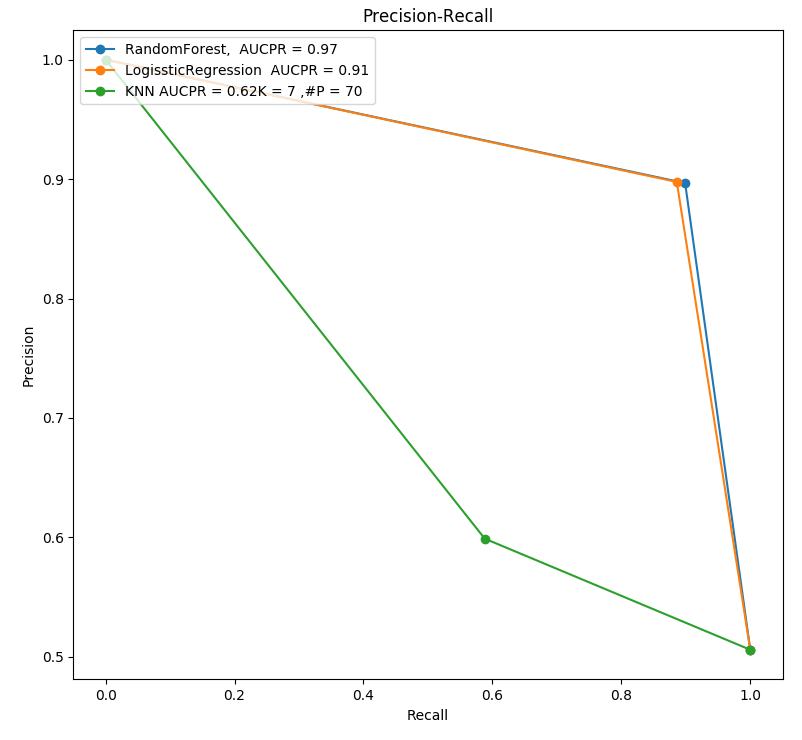
\includegraphics[scale=.25]{ALLModels.png} %{with .png} 
\end{center}
Fig. 7 AUCPR of the best model for each of the selected methods. 

\begin{table}[H]
\begin{tabular}{|l|l|l|l|}
\hline
                        & \textbf{RF} & \textbf{LOG} & \textbf{KNN} \\ \hline
\textbf{Execution Time (Seconds)} & 160         & 0.594        & 570          \\ \hline
\textbf{Mean}           & 0.96        & 0.88         & 0.6          \\ \hline
\textbf{STD}            & 0.01        & 0.04         & 0.01         \\ \hline
\end{tabular}
\end{table}
Table 1  Summary of the best selected models 

\section{Conclusion}  
Determining the best classifier for any given data is not an easy and trivial task to perform. Multiple cross validation procedures, feature selection, and parameter tuning must be done to be able to find the best, or at least a very good model, to use for the proper classification of the data. Since every permutation of features and parameters cannot be tested for all the possible models in every single case, computer scientist and engineers must be very careful about how they perform their model selection and training. In this assignment, KNN, random forest and logistic regression were tested to determine the best possible model, and for this particular instance, random forest yielded the best results. 


\end{document}